\documentclass{report}
\usepackage{fullpage}
\usepackage[margin=0.75in]{geometry}
\usepackage{hyperref}
\usepackage{amsfonts}
\usepackage{float}
\usepackage{graphicx}
\usepackage{caption}
\usepackage{subcaption}
\usepackage{color}
\renewcommand{\baselinestretch}{1.5}
\author{Steven Englehardt, Maciej Halber, Elena Sizikova}
\title{Understanding Collections of Images \\ \small{COS 521 Final Project Report}}
\begin{document}
\maketitle
\tableofcontents

\chapter{Introduction}
\section{Abstract}
This report explores a variety of image properties which make it possible to understand and explore collections of images. In particular, we look at how properties like color distribution, saturation, sharpness, and detail can be extracted and compared between images. To extract these features we make use of the Fast Fourier Transform (FFT) and Singular Value Decomposition (SVD) of images. We seek to understand how the theoretical underpinnings of these two algorithms affect the way these algorithms transform images and use that to gain an understanding of the fundamental components of an image. Ultimately, we test our understanding of images by creating a concise mathematical notation (a descriptor) from image fundamentals and test how well it differentiates between a collection of images.

\section{Background Work}
{\color{red} I'll look at this section closer tmrw, definietly needs some expanding. Will add some color histogram stuff  -- Maciej}

{\color{red} This is kinda a merged background/motivation section. We should either give some background work for SVD and FFT (citations to other papers) or make it primarily a motivation section. -- Steve}

There are many possible situations in which we would need to understand and compare image structure. For example, one might like to search for a location in which a photograph was taken, by looking at all the other available images, and finding the image closest to the search image. Alternatively, one may want to cluster images based on their content, and see what categories the image collection can be decomposed to. Both of these would be easy problems to solve, if the images were annotated with words; textual search is a well-solved problem. However, when the images are not labelled and the collection size is extremely large, it is impractical to label by hand. For such problems, it is important to have a model to summarize image content automatically.

Existing methods of image search by analyzing content of the image include Google Goggles and Google Image Search, both are based on similar technology \cite{google_blog}, which checks for distinctive points, analyzes lines and textures to create a mathematical model of the image. {\color{red} While the exact implementation is not available, Google Image Search does not provide clustering capabilities of analyzing existing input datasets. [[not sure what this is trying to say?]]} A more relevant study is that of Oliva and Torralba \cite{gist_descriptor} which creates a GIST descriptor {\color{red}(cite Freedmans work!!!)}, and uses perceptual dimensions (e.g. naturalness, openness, roughness, expansion, ruggedness) to classify natural images (e.g. pictures of coasts, mountains, or cities). The author's work with a low dimensional representation of a scene is collectively known as the \emph{Spatial Envelope}. The properties of the spatial envelope are estimated by means of Discrete Fourier Transform (DFT), Windowed Fourier transform (WFT), as well as spectral properties of the image are estimates {\color{red}(!!!! Expand)}. 

Having completed a graduate course in algorithms, our goal was to understand the results of such a study, and specifically answer the question: why can we estimate properties of the spatial envelope the way \cite{gist_descriptor} does? 


\chapter{Methods}
In this project, we analyze image structure from three directions: color distribution, frequency distribution, and geometrical structure. An analysis of image color distribution is given in section \ref{sec:color}. The properties of images after transformation to the frequency domain by FFT are explored in section \ref{sec:FFT}. Images decomposed with SVD are studied in section \ref{sec:SVD}, to discover underlying geometrical structure.
 
%   We first started with a collection of color images that were analyzed by the method of Color Histograms. We also analyzed the properties of the FFT method and the SVD method on the corresponding greyscale images. The resulting descriptors were then compared against each other and subsequently combined into a joint descriptor, that used the information from all three methods to describe images.

\section{Data}
The dataset that we have used for exploring image structure has been provided by Oliva and Torralba \cite{gist_descriptor}. The dataset contains images labelled as one of 8 outdoor scene categories: coast, mountain, forest, open country, street, inside city, tall buildings and highways. There are 2600 256x256 color images in jpg. The images in the dataset are varied in complexity: from very simple, planar scenes (e.g. a ground and sky) to very complex and busy images (e.g. cars, people, and buildings in a city). This dataset was chosen because it provides a full range of colors, complexities, and textures, and because image categories allow us to easily pick images with similar physical content.

\section{Implementation}

When decomposing images using SVD or working with the FFT of an image, we chose to work in grayscale. The choice to do so was motivated by the desire to explore the physical meaning of the decomposition or transformation in the context of images. Though it is entirely possible to separate the red, green, and blue channels and work with each separately, it is difficult to determine whether relative differences in colors or deeper properties of the decomposition/transformation are leading to the observed descriptor performance. To do the conversion we used matlab's built-in \textit{rgb2gray} function, which removes hue and saturation information but preserves luminance. {\color{red} Above sentence is not exactly true - recovering luminance vs preserving color is a huge area of work, basically look up for integral images if interested. Will have to tweak the section a bit -- [Steve] - that sentence was lifted from the matlab documentation, see: \url{http://www.mathworks.com/help/images/ref/rgb2gray.html}, that is the extent of my knowledge, so feel free to update.}

\section{Color Analysis}
\label{sec:color}
\subsection{Color Spaces}
\label{sec:colorSpaces}
% The subset of image colors that can be seen on a computer monitor are known as \emph{gamut}, see \cite{color_model_ref}. As we only considered computer images in .jpg and .png formats, we were mainly concerned with the models that represent the gamut. 
In computer graphics the subset of colors which can be displayed by computer monitor is called \emph{gamut}\cite{color_model_ref}. There are many models which aim to represent the gamut --- one of the most common and well known such models is known as the RGB model, in which color at every pixel is a combination of three intensity values, of the Red, Green, and Blue base colors. RGB models how devices produce colors, so our initial intuition was to look at models that model human vision more closely.  
\begin{figure}[hbtp]
\centering
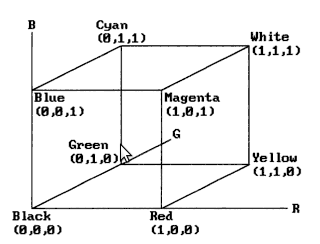
\includegraphics[scale=0.5]{graphics/rgb_cube.png}
\caption{RGB Cube Model}
\end{figure}

One of such models is Hue-Saturation-Value model, which were designed to give more intuitive in terms of human color perception, and thus is widely used as color picker in many photo-editing and digital painting packages \cite{color_model_ref}.
HSV model is a fairly straightforward transformation from the RGB model, as shown in \ref{fig:hsv_visualisation}.

\begin{figure}[hbtp]
        \centering
        \begin{subfigure}[b]{0.3\textwidth}
                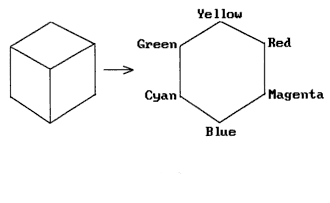
\includegraphics[width=\textwidth]{graphics/hsv_cube.png}
                \caption{The RGB cube viewed along Black-White diagonal}
                \label{fig:gull}
        \end{subfigure}%
        ~
         %add desired spacing between images, e. g. ~, \quad, \qquad etc.
          %(or a blank line to force the subfigure onto a new line)
        \begin{subfigure}[b]{0.3\textwidth}
                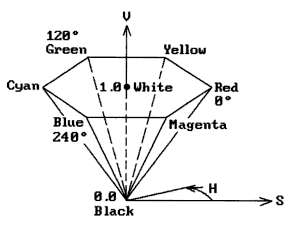
\includegraphics[width=\textwidth]{graphics/hsv_rescale1.png}
                \caption{Recoordination}
                \label{fig:mouse}
        \end{subfigure}
        ~
         %add desired spacing between images, e. g. ~, \quad, \qquad etc.
          %(or a blank line to force the subfigure onto a new line)
        \begin{subfigure}[b]{0.3\textwidth}
                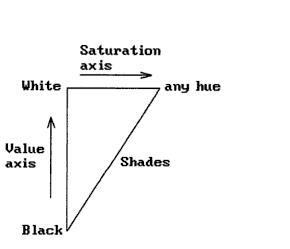
\includegraphics[width=\textwidth]{graphics/hsv_rescale2.png}
                \caption{Hue-Saturation Triangle}
                \label{fig:tiger}
        \end{subfigure}
        \caption{Transformation of the RGB cube to HSV color space}\label{fig:hsv_visualisation}
\end{figure}

In particular, the hue varies from $0^{\circ}$ to $360^{\circ}$, and represents the color. The saturation and value are numbers in the range $[0,1]$ which represent how far is the hue from white and black, respectively. \\

{\color{red} @Elena - if you have some nice figure for L*a*b we can put it here}\\

Another color space which we have considered in this work was the $L^*a^*b^*$ color space which also has been designed to model the human perception closely. $L^*$ parameter control the overall lightness of the image, ranging from $L=0$ being black, and $L=100$ yielding white. Both $a^*$ and $b^*$ range from negative to positive values, where negative $a*$ yields, and positive values give colors closer magenta. For $b*$ negative values give blue color, while positive values relate to yellow. Since $L^*a^*b^*$ aims to be most complete color model that represents all colors that are perceived by human vision it was a clear choice to investigate what improvements we might get from the incorporation L*a*b* in our color descriptors, which will be introduced in next section.

\subsection{Color-based Descriptors}
The color information is widely used for image retrial, since as a descriptor it has a nice properties of being rotationally invariant, as well as not being dependent on image resolution. As mentioned in previous section, color closely relate to how we percieve images as similar. Also similar objects will yield similar colors, especially in terms of natural objects ( i.e. forest images will always be mostly green, landscapes will always show a blue sky etc. ). 

A very crude way of comparing images in terms of colors is to average each of the channels in specific color space, and use it as a $3$-value descriptor, which will be a point in a color space. Figure \ref{fig:colSpaces} shows points plotted in $\mathbb{R}_3$. What is interesting about all the color spaces is the fact that we can easily navigate through them and have a good understanding how single parameter affects overall color appearance.

\begin{figure}[hbtp]
\centering
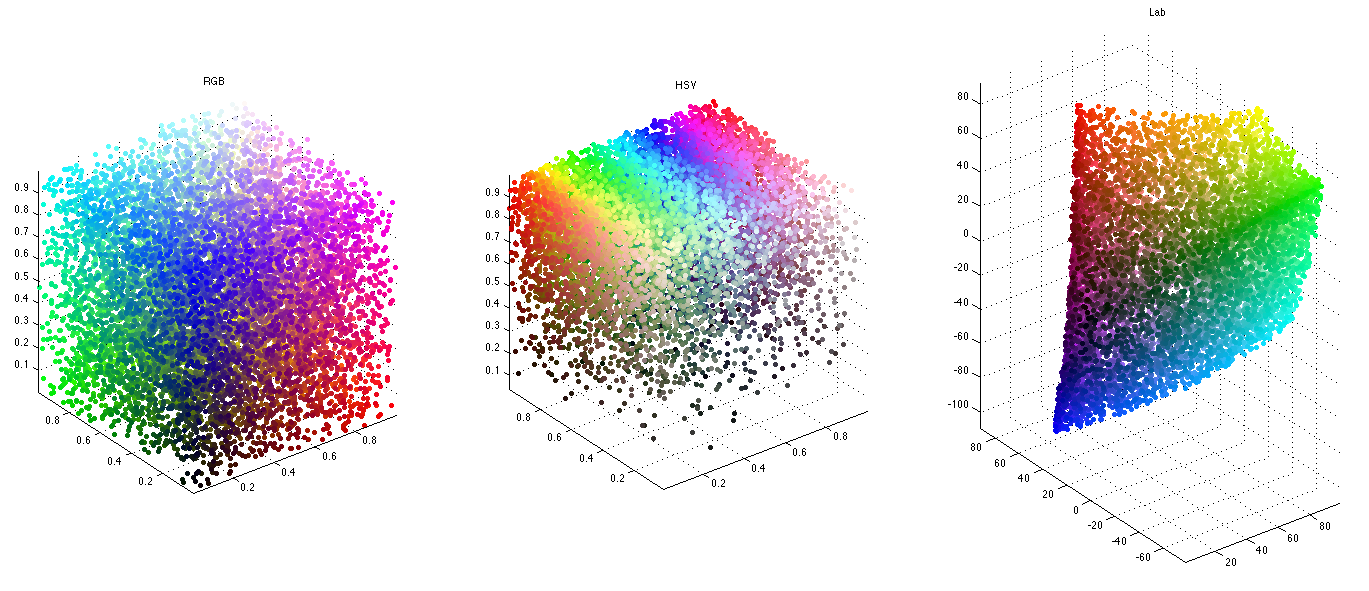
\includegraphics[scale=0.3]{graphics/colorSpaces.png}
\caption{Points in $\mathbb{R}_3$, plotted according to their values in RGB, HSV and $L^*a^*b^*$ color spaces }
\label{fig:colSpaces}
\end{figure}

This gave us the inspiration to look for similar, simple parameters that relate to overall image structure, using FFT and SVD ( see sections \ref{sec:FFT} and \ref{sec:SVD} respectively). However by a simple averaging we are not obtaining information regarding the overall color distribution. A more common way of investigating the color distribution is \textit{normalized color histogram}. To create it we first create bins - given the number of bins $n$ we create a set of uniformly spaced ranges $R = \{r_1, r_2, ..., r_n\}$. Now for each pixel $p_i$ we determine its value $v_i$ and determine into which $r_k$ it falls to and increment value at the relating bin. After visiting all pixels $p_i$ we normalize each bin by total number of pixels. This produces a length $n$ vector that better describe the the overall value distribution. Above structure of course describes the procedure for gray scale images, however it is trivial to extend it to color images where we create a histogram for each color channel, and then concatenate resulting vectors.

\begin{figure}[hbtp]
\centering
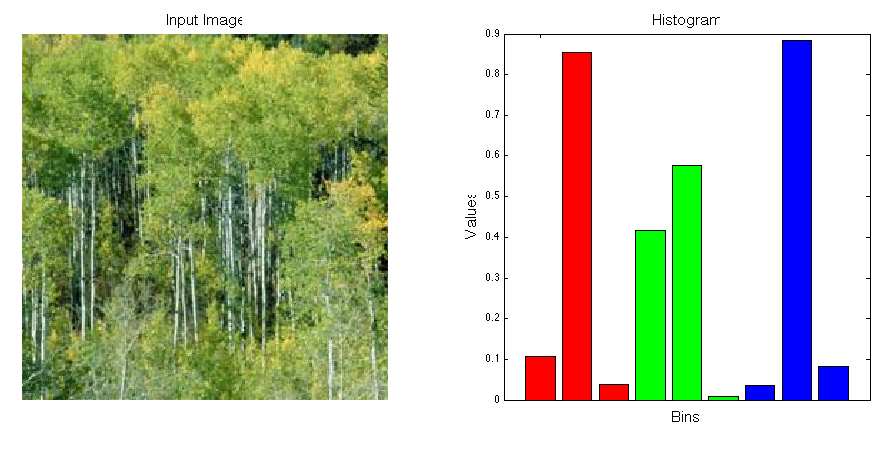
\includegraphics[scale=0.3]{graphics/colorHistogram.png}
\caption{Image and its color histogram in RGB, with $n = 3$ bins per channel. }
\label{fig:colSpaces}
\end{figure}

We then designed our descriptor for each color space. As noted in \cite{HSV_non_uniform}, hue is more important for color perception than saturation and lightness, and thus the HSV histogram have been always computed giving more bins to hue channel (i.e. provided that the required length of descriptor is $n$, the number of bins for hue would be given by $\frac{n}{2}$, while other two parameters $\frac{n}{4}$. Similarly we conjecture that in terms of $L^*a^*b^*$ color space the lightness is less important than parameters describing colors, so we have also modified the number of bins for each channel accordingly ( $L^* = \frac{2*n}{8}$,$ a^* = \frac{3*n}{8}$, $b^* = \frac{3*n}{8}$ )

To sum up for color descriptors we have looked both at simple averaging of values as well as normalized color histograms. All these have been implemented to work with each of the color spaces discussed in section \ref{sec:colorSpaces}. In chapter \ref{chap:analysis} we discuss the overall performance of all descriptors discussed here. Also note that in literature it is common to note that uniform quantization does not take the spatial relationship between pixels into account, and investigate the techniques to overcome this drawback \cite{GaussQunatization}. However because of time limitation we have decided to settle for simpler approach.

\section{Fourier Transform} 
\label{sec:FFT} 
A $2$-dimensional, Discrete Fourier Transform(DFT) of an grayscale image is a transformation from the spatial domain to the frequency domain. In the spatial domain, image is represented by function $f(x,y)$ on all relevant points $(x,y)$ in  $\mathbb{R}^2$. In the frequncy domain, the image is represented by a function $F(u,v)$ where $u$ and $v$ are frequency values. It follows that in the frequency decomposition, an image is represented by a matrix of complex values $F$, where $F(u,v)$ encodes the amplitude and the phase of the frequencies $u$ and $v$. Mathematically, the $2$-D Fourier Transform is defined as:
\begin{eqnarray}
F(u,v) = \int \int ^{\infty}_{-\infty} f(x,y)e^{-j2\pi (ux+vy)}dx dy
\end{eqnarray}
For $n$ points, we can compute the $1$-D DFT efficiently in $O(n\log{n})$ operations. The Matlab implements $2$-D FFT  in funcion \textit{fft2}, which is extremely  fast, and we had no computational time issues when basing our descriptors on these computations.

\subsection{Amplitude and Phase Analysis}
Consider the decomposition of an image of a building in a city from the GIST dataset into its power(amplitude) and phase spectra.
\begin{figure}[H]
        \centering
        \begin{subfigure}[b]{0.2\textwidth}
                
\includegraphics[width=\textwidth]{graphics/original.png}
                \caption{Original image}
                \label{fig:gull}
        \end{subfigure}%
        ~
         %add desired spacing between images, e. g. ~, \quad, \qquad etc.
          %(or a blank line to force the subfigure onto a new line)
        \begin{subfigure}[b]{0.2\textwidth}
                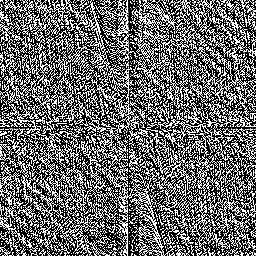
\includegraphics[width=\textwidth]{graphics/phase.png}
                \caption{Phase $\Phi(x,y)$}
                \label{fig:mouse}
        \end{subfigure}
        ~
         %add desired spacing between images, e. g. ~, \quad, \qquad etc.
          %(or a blank line to force the subfigure onto a new line)
        \begin{subfigure}[b]{0.2\textwidth}
                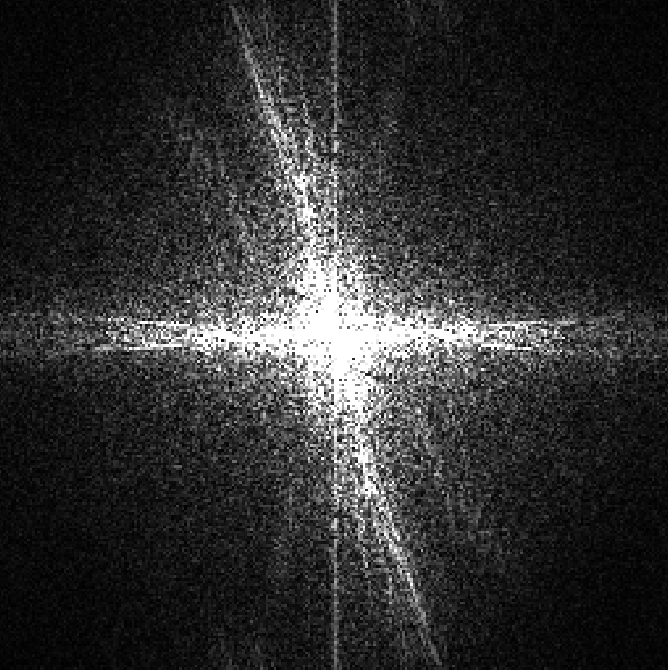
\includegraphics[width=\textwidth]{graphics/ampl.png}
                \caption{Amplitude $A(x,y)$}
                \label{fig:tiger}
        \end{subfigure}
%        ~
%        \begin{subfigure}[b]{0.2\textwidth}
%                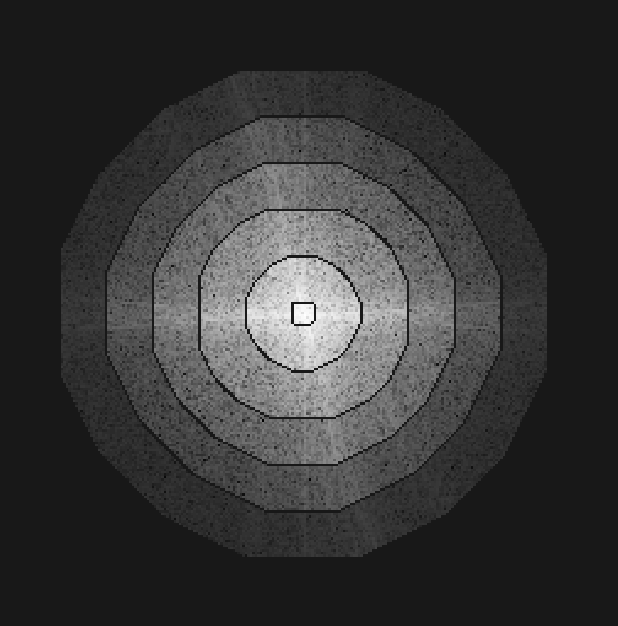
\includegraphics[width=\textwidth]{graphics/freq_bins.png}
%                \caption{Frequency Bins}
%                \label{fig:mouse}
%        \end{subfigure}
        \caption{Phase and power spectra of building image}\label{fig:fft_localization}
\end{figure}
As Oliva writes in \cite{gist_descriptor}, the phase image represents local properties of the image. It contains information relative to the form and the position of image components. This can be further understood by taking the true phase values of the image, and setting all the amplitude values to $1$ (effectively taking out all amplitude variation and flattening the image), or taking true amplitude values and randomizing the phase:
\begin{figure}[H]
        \centering
        \begin{subfigure}[b]{0.2\textwidth}
                
\includegraphics[width=\textwidth]{graphics/original.png}
                \caption{Original image}
                \label{fig:gull}
        \end{subfigure}%
        ~
         %add desired spacing between images, e. g. ~, \quad, \qquad etc.
          %(or a blank line to force the subfigure onto a new line)
        \begin{subfigure}[b]{0.2\textwidth}
                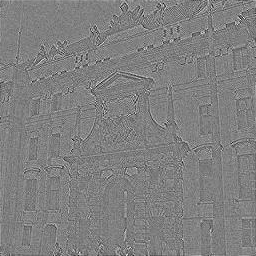
\includegraphics[width=\textwidth]{graphics/flat_power.jpg}
                \caption{Flat amplitude}
                \label{fig:mouse}
        \end{subfigure}
        ~
         %add desired spacing between images, e. g. ~, \quad, \qquad etc.
          %(or a blank line to force the subfigure onto a new line)
        \begin{subfigure}[b]{0.2\textwidth}
                
\includegraphics[width=\textwidth]{graphics/randomized_phase.jpg}
                \caption{Randomized phase}
                \label{fig:tiger}
        \end{subfigure}
        \caption{Analysis of Contributions of both Phase and Amplitude to an Image}\label{fig:fft_randomization}
\end{figure}
Note that a reconstructed image in which the amplitude information was not preserved retains the information about the edges and outlines in the original image. However, after Oliva \cite{gist_descriptor}, the amplitude image (power spectra) informs us on global properties of the image structure, telling us about the orientation, smoothness, lenght and strenght of the edges that appear in the image.
Two images that are similar might have different local information in terms of contours appearing in them, however they should have similar power spectra. This insight motivates our decision to investigate the amplitude image for our descriptor, since our goal is do capture the global properties of the image.

\subsection{Localization fact}
To understand the properties of the $2$-D Fourier Transform more deeply, let us first analyze the $1$-D variant first. Consider the following functions, and their representations in the Fourier domain (\ref{fig:fft_localization}). A plot of $f(x)=\cos {x}$ is not very well localized in the spatial domain, that is, we can inutitively state that function is streteched along the x-axis. In more mathematical terms we can say that a small change in the function domain $\delta_x$ relates to small change $\delta_y$ in the function image.  However, when we analyze same function in the Fourier domain, we notice that its representation is extremly packed --- for $F(cos(x))$, the representation is just a single peak. Conversely, $g(x)=\cos {50x}$ is well localized in the spatial domain, i.e. function can be thought of being squeezed along x-axis. Again, more strict definition would be that small change in the function domain $\delta_x$, relates to dramatic change$\delta_y$, i.e. $\delta_y \gg \delta_x$. However, in the Fourier domain, we observe inverted behaviour - the peaks of the $F(g(x))$ spread apart away from the zero frequency. This simple fact regarding the behavior of Fourier Transfrom suggested us a way of how to describes images in the Fourier domain, analyzing its amplitude image $A(x,y)$. Images containing a lot of high frequency periodicy (buildings, trees) will have more contribution from these (high) frequencies, while images showing open landscapes will mostly consist of low frequencies. Similarly to our approach with color descriptors, we can try to generate bins of different frequencies, and then normalize them to get overall contribution from each frequency range.

\begin{figure}[h]
        \centering
        \begin{subfigure}[b]{0.2\textwidth}
                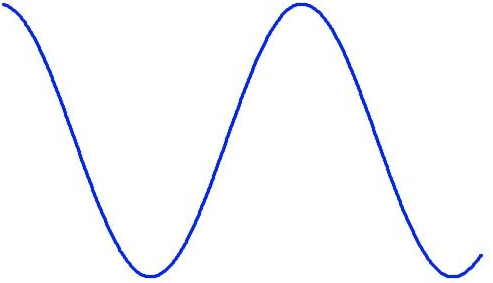
\includegraphics[width=\textwidth]{graphics/graph_fft_1.jpg}
                \caption{$f(x)=\cos{x}$}
                \label{fig:gull}
        \end{subfigure}%
        ~
         %add desired spacing between images, e. g. ~, \quad, \qquad etc.
          %(or a blank line to force the subfigure onto a new line)
        \begin{subfigure}[b]{0.2\textwidth}
                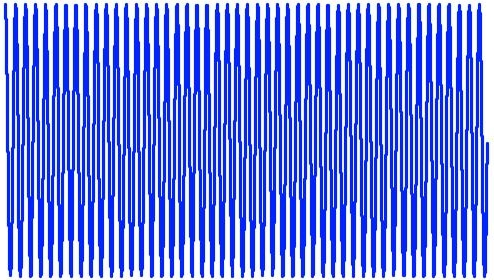
\includegraphics[width=\textwidth]{graphics/graph_fft_2.jpg}
                \caption{$g(x)=\cos{50x}$}
                \label{fig:tiger}
        \end{subfigure}
        
         %add desired spacing between images, e. g. ~, \quad, \qquad etc.
          %(or a blank line to force the subfigure onto a new line)
        \begin{subfigure}[b]{0.2\textwidth}
                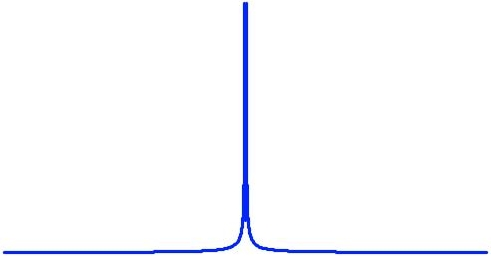
\includegraphics[width=\textwidth]{graphics/graph_fft_3.jpg}
                \caption{$F(f(x))$}
                \label{fig:mouse}
        \end{subfigure}
        ~
        \begin{subfigure}[b]{0.2\textwidth}
                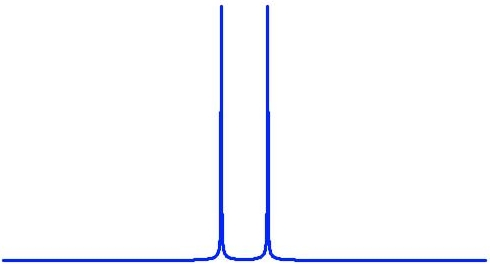
\includegraphics[width=\textwidth]{graphics/graph_fft_4.jpg}
                \caption{$F(g(x))$}
                \label{fig:mouse}
        \end{subfigure}
        \caption{Example of localization properties of different functions in the spatial and Fourier domains. Images localized in the spatial domain are not localized in the Fourier domain, and vice versa.}\label{fig:fft_localization}
\end{figure}

To test the above analysis we have created a simple, single-value descriptor, that was just looking at the contribution from the low frequencies - the descriptor $d(I)$ is simply given by :
$$
d(I) = \sum_{x^2 + y^2\in{r_0}}A(x,y)
$$
where $r_0 = \{0, \omega_1\}$ is a range of frequencies from zero to some small frequency $\omega_1$. Idea is again that images with lots of high frequency information, will have less contribution from low frequencies, and thus returning smaller value $d(I)$. We sorted the images according the increasing contribution of low frequencies \ref{fig:fft_low_freq_order}. The images should be read as one line that starts at top-left corner and ends in bottom-right. 

\begin{figure}[hbtp]
\centering
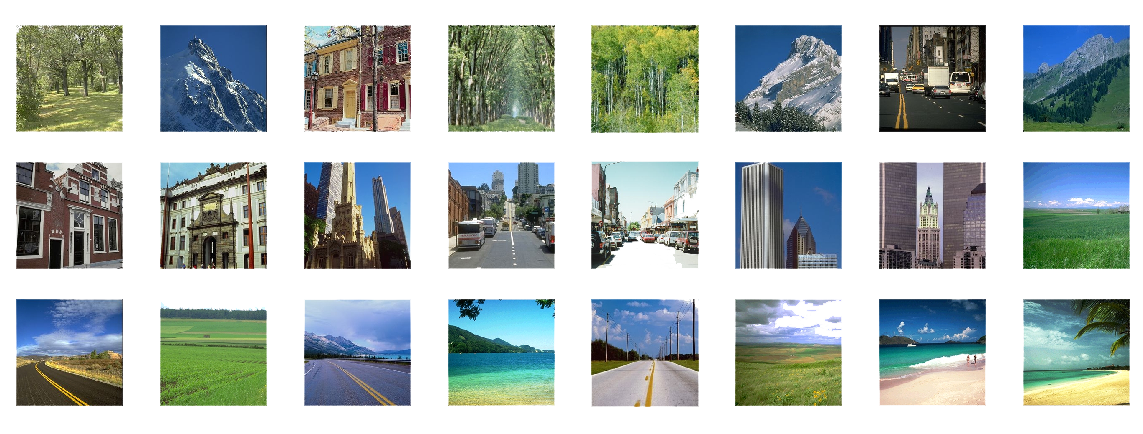
\includegraphics[scale=0.3]{graphics/FrequencyOrdered.png}
\caption{Ordering of a subset of the dataset by increasing contribution of low frequencies}
\label{fig:fft_low_freq_order}
\end{figure}

One can see that the images on the left side of the spectrum, with a lot of contribution from high frequencies and not so much from low frequencies have many small details: they show leaves, rock incisions on the mountain, and fine building facade. In comparison, the images at the right side of the spectrum are images of open country, roads, and beaches. These images are simple, in the sense that they have a dominant horizon line and not so much small detail. It follows that these images are described mostly by low frequencies, and not by high frequencies. Notice that this analysis discards a lot of information about the distribution of frequency contribution.

\subsection{Frequency-Based Descriptor}
Given that simple descriptor described in the previous section allowed us to create quite meaningful ordering of images we decided to extend it to give us better information regarding the overall frequency distribution, similarly to our color descriptors. The said extension, simply consider a set of disjoint, uniformly spaced, frequency ranges $\{r_0, r_1, ..., r_n\}$, see fig. \ref{fig:freqDescriptor}.   
\begin{figure}[hbtp]
\centering
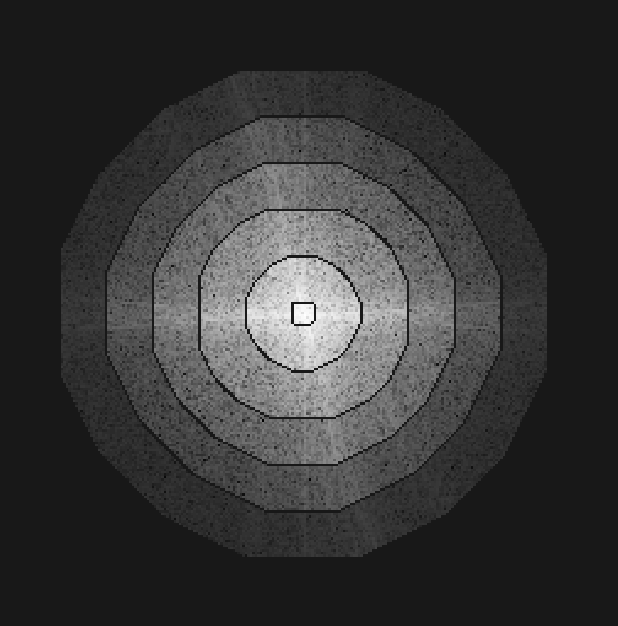
\includegraphics[scale=0.3]{graphics/freq_bins.png}
\caption{Frequency Descripor Visualization}
\label{fig:freqDescriptor}
\end{figure}

Our descirptor is then a vector $\vec{d}(I)$, of n-values, where each value is simple averaging of frequency values in specific bin, that is then normalized by $N = \sum_x,y A(x,y)$, the averaging of all values in an image. This way, each element $d_i$ give us percentage contribution from each frequency range. We will discuss the performance in chapter \ref{chap:analysis}.\\

{\color{red}Or add the figures with performance here}

\section{Singular Value Decomposition}
\label{sec:SVD}
A deeper understanding of Singular Value Decomposition (SVD) in the context of images allows the creation of a descriptor that captures overall image complexity in a relatively small descriptor length. SVD is a factorization of any real or complex 2-dimensional matrix. Since images will always be represented by real matrices, we ignore the complex case in our analysis. 

Consider an $m \times n$ matrix $A$. The singular values of $A$  correspond to the non-zero square roots of the eigenvalues from $AA^T$ and $A^TA$. The matrix $AA^T$ is spanned by the row space of A, and the matrix $A^TA$ is spanned by the column space of $A$ \cite{using_svd}. The row space and column space being the set of all linear combinations of row vectors and column vectors of $A$, respectively.

SVD conveniently decomposes $A$, separating out singular values, row space eigenvectors, and column space eigenvectors into three different matrices. The SVD of $A$ is defined as:
$$A_{\scriptscriptstyle m \times n} = U_{\scriptscriptstyle m \times m}S_{\scriptscriptstyle m \times n}V_{\scriptscriptstyle n \times n}^T$$
where $S$ is a diagonal $m \times n$ matrix with the singular values of $A$ on the main diagonal (in decreasing order). The columns of $U$ are the eigenvectors of $AA^T$ and the columns of $V$ are the eigenvectors of $A^TA$ \cite{using_svd}. $U$ and $V$ are known as the left and right singular vectors of $A$, respectively.

The rank of a matrix is informally defined as a measure of the "nondegenerateness" of system of linear equations encoded by that matrix, or more formally is equal to the size of the row space or column space of the matrix. Linearly independent singular vectors correspond to non-degenerate singular values.  The rank of a matrix is thus equal to the number of non-degenerate singular values of the matrix, and is also equal to the number of linearly independent vectors in $U$ or in $V$. If all singular values are non-degenerate, $A$ is a full rank matrix and the SVD of $A$ is unique.

\subsection{SVD and Compression}
It is useful to think of each singular value in $S$ as scaling the row and column singular vectors from $U$ and $V$ to generate an 'eigenimage' \cite{svd_image_coding}, or the contribution of that specific singular value to the overall image. This construction is what enables image compression through a low-rank matrix approximation. Let $\tilde{A}$ represent the $k$-approximation of $A$, where $rank(\tilde{A}) = k$. Thus:
$$\tilde{A} = U(:,1:k)\tilde{S}V(:,1:k)^T$$

\begin{figure}[H]
        \centering
        \begin{subfigure}[b]{0.4\textwidth}
                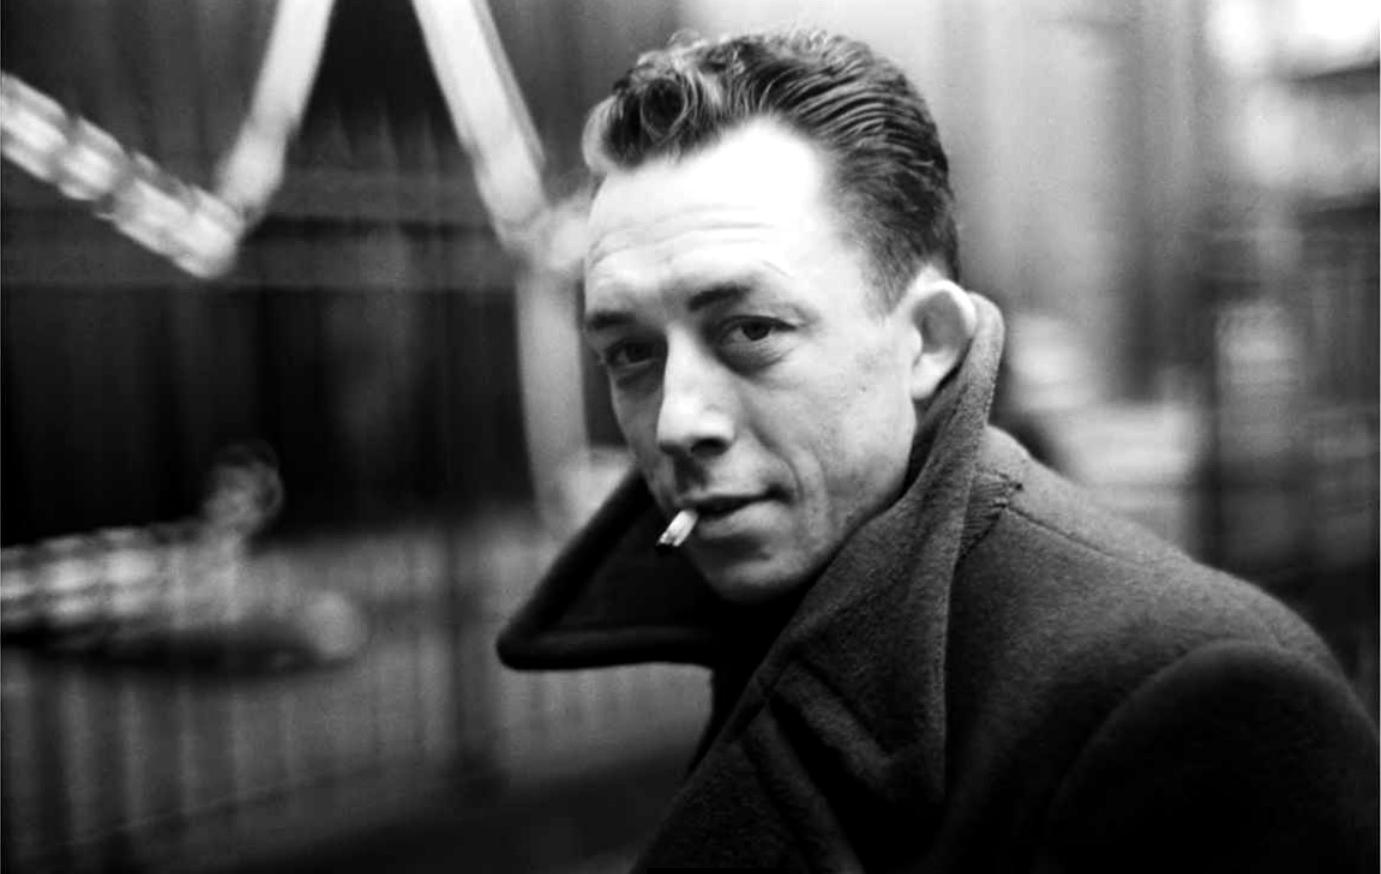
\includegraphics[width=\textwidth]{graphics/guy.jpg}
                \caption{Original image}
        \end{subfigure}
        \begin{subfigure}[b]{0.4\textwidth}
                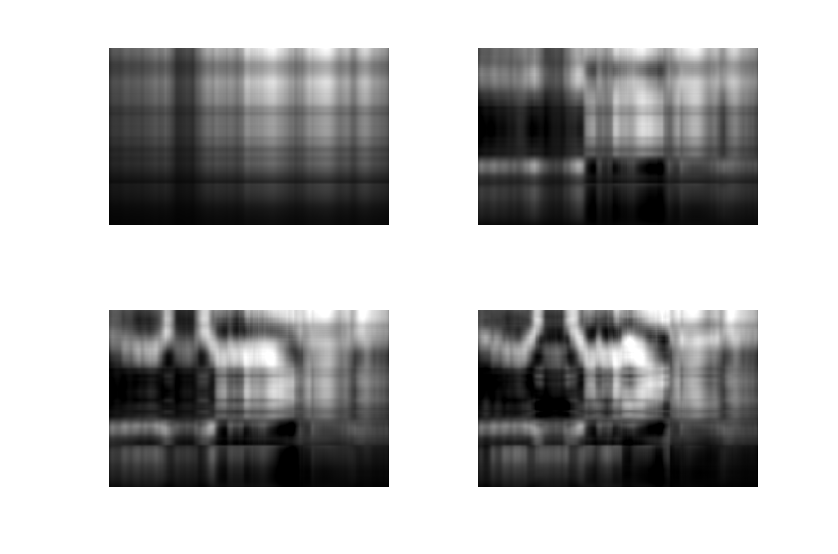
\includegraphics[width=\textwidth]{graphics/guyTopCompressions.png}
                \caption{Rank 1 to 4 from top left to bottom right}
        \end{subfigure}
        \caption{Rank k-approximations of an image using SVD}\label{fig:svd_compression}
\end{figure}

The performance of SVD in image compression shows that there is a significant amount of visual information in low rank approximations of images. Our desire is to capture this low rank information in a concise descriptor for use in image retrieval. An examination of both the singular values and the singular vectors follows.

\subsection{Singular Values}

Image retrieval using all singular values of a matrix has been shown to perform better than a simple distance metric, such as the Mahalanobis distance, Manhattan distance, or Euclidean distance \cite{svd_image_retrieval}. Several factors contribute to this performance, but relate to the fact that the distribution of singular values in $S$ is connected to the rank of $A$, the image matrix. 

The alignment of an images' strongest color contours to either the horizontal or vertical axis allow it to be fully captured in the left or right singular vectors of an image and thus requires few singular values. The means the image's matrix representation is of lower rank and thus loses less information by ignoring the smallest singular values. In an extreme example, the three images in Figure \ref{fig:rank1_images} can be fully represented using only the top singular value since they are all rank 1 matrices.

\begin{figure}[H]
        \centering
        \begin{subfigure}[b]{0.2\textwidth}
                
\includegraphics[width=\textwidth]{graphics/horizontalGrad.png}
                \caption{$S(1,1) = 37726$}
        \end{subfigure}
        ~~~
        \begin{subfigure}[b]{0.2\textwidth}
        		
\includegraphics[width=\textwidth]{graphics/smallVertical.png}
        		\caption{$S(1,1) = 46041$}
        \end{subfigure}
        ~~~
        \begin{subfigure}[b]{0.2\textwidth}
                
\includegraphics[width=\textwidth]{graphics/smallHorizontal.png}
                \caption{$S(1,1) = 46041$}
        \end{subfigure}
        \caption{Rank 1 images and their top singular value}
        \label{fig:rank1_images}
\end{figure}

On the opposite end of the spectrum, consider the randomly generated images in Figure \ref{fig:rand_images}. These three images are full rank and require all 256 singular values for a full reconstruction. The plot of the singular values from these images reveals that the range of intensity in the image directly correlates to the magnitude of the singular values needed, but has no correlation to the number of values needed.

\begin{figure}[H]
        \centering
        \begin{subfigure}[b]{0.2\textwidth}
                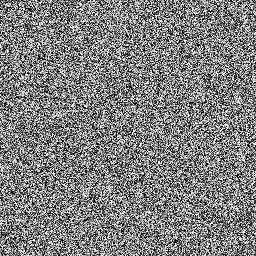
\includegraphics[width=\textwidth]{graphics/randomFullSpace.png}
                \caption{Full: $0-255$}
        \end{subfigure}
        ~~~
        \begin{subfigure}[b]{0.2\textwidth}
        		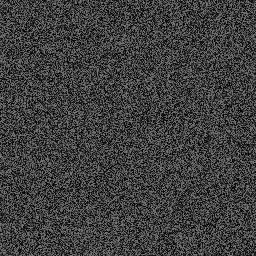
\includegraphics[width=\textwidth]{graphics/randomBottomHalfSpace.png}
        		\caption{Half: $0-127$}
        \end{subfigure}
        ~~~
        \begin{subfigure}[b]{0.2\textwidth}
                
\includegraphics[width=\textwidth]{graphics/randomBottomQuarterSpace.png}
                \caption{Quarter: $0-63$}
        \end{subfigure}

        \begin{subfigure}[b]{0.6\textwidth}
                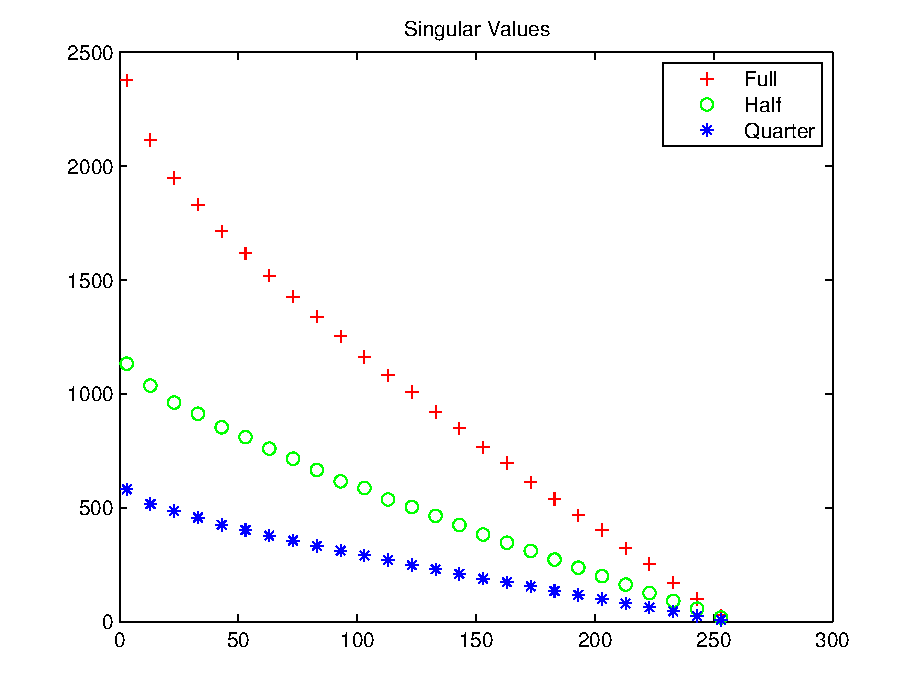
\includegraphics[width=\textwidth]{graphics/singular_values_color_space.pdf}
                \caption{Plot of singular values (1st value omitted for scaling)}
        \end{subfigure}
        \caption{(a-c): Random images with given intensity range (d): Singular values of (a-c)}
        \label{fig:rand_images}
\end{figure}

Figure \ref{fig:rank1_images} shows very simple rank 1 images that only require the 1st singular value, whereas Figure \ref{fig:rand_images} shows that full rank images requires all singular values. To get a better understanding of the required number of singular values we look at what happens when there is symmetry in the image. Figure \ref{fig:rand_symmetry} shows the plot of singular values from several random images which span the full intensity range from $0-255$, but have symmetry in various directions. In all images, the symmetry is about a central axis, so it covers half of the image.

\begin{figure}[H]
        \centering
        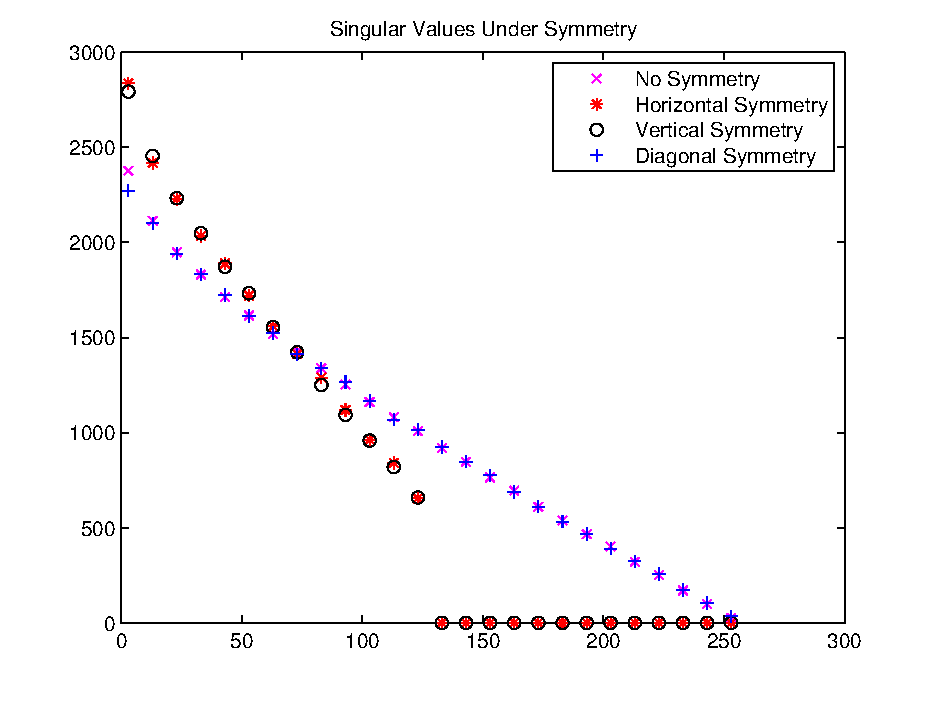
\includegraphics[width=0.6\textwidth]{graphics/singular_values_symmetry.pdf}
        \caption{Plot of singular values under symmetry (1st value omitted for scaling)}
        \label{fig:rand_symmetry}
\end{figure}

Figure \ref{fig:rand_symmetry} shows that the amount of symmetry within an image can greatly reduce the number of singular values required for reconstruction (in this case by half, since half of the image was repeated). The direction of symmetry along the horizontal or vertical axis has very little affect on the distribution of singular values. However, an image which has symmetry off-axis at a $45^\circ$ angle will still have linearly independent vectors in $U$ and $V$ as the image is still full rank. Despite the fact that half of the image is repeated, the distribution of singular values is nearly identical to the image with no symmetry. It should be noted that $45^\circ$ is chosen because it represents the worst-case off-axis example. Angles above and below will experience some level of symmetry in either the horizontal or vertical direction.

\begin{figure}[H]
        \centering
        \begin{subfigure}[b]{0.17\textwidth}
                \begin{subfigure}[H]{\textwidth}
                	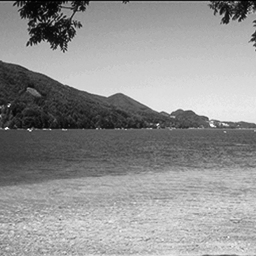
\includegraphics[width=\textwidth]{graphics/coast.png}
                	\caption{Coast}
        		\end{subfigure}
        		\begin{subfigure}[b]{\textwidth}
        			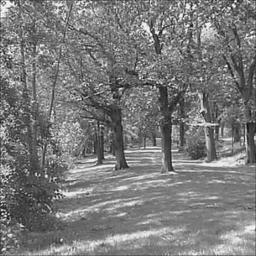
\includegraphics[width=\textwidth]{graphics/forest.png}
        			\caption{Forest}
        		\end{subfigure}
        \end{subfigure}
        ~
        \begin{subfigure}[b]{0.17\textwidth}
        		\begin{subfigure}[b]{\textwidth}
                	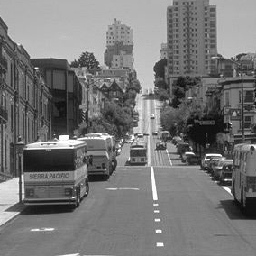
\includegraphics[width=\textwidth]{graphics/street.png}
                	\caption{Street}
        		\end{subfigure}
        		\begin{subfigure}[b]{\textwidth}
        			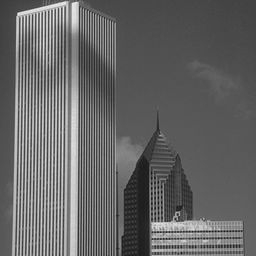
\includegraphics[width=\textwidth]{graphics/tallbuilding.png}
        			\caption{Building}
        		\end{subfigure}
        \end{subfigure}
        \begin{subfigure}[b]{0.55\textwidth}
                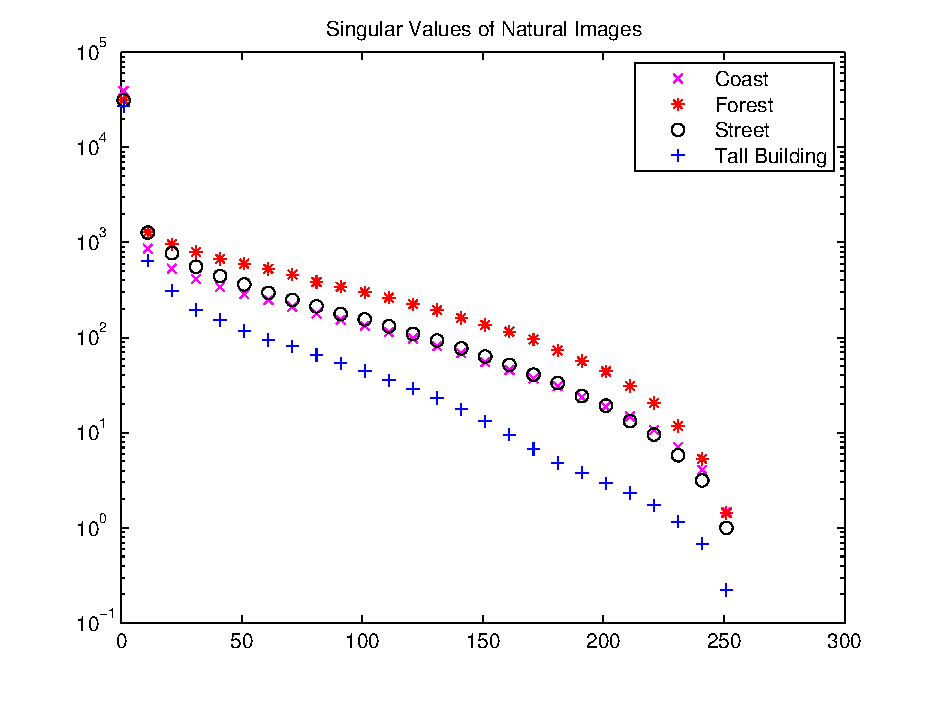
\includegraphics[width=\textwidth]{graphics/singular_values_natural_images_log.pdf}
                \caption{Plot of singular values (log-scale)}
        \end{subfigure}
        \caption{Examination of singular values for natural image classes}
        \label{fig:singular_values_natural}
\end{figure}

Figure \ref{fig:singular_values_natural} shows a sample of the distribution of singular values for natural images which vary quite a bit in terms of complexity and repeated structure within the image. Images with high repeated structure aligned to the horizontal (a,c) or vertical (d) direction decay more quickly than images with less repeated structure (b). Despite being similar in the repeated structure of the image, the coast and street images are quite different otherwise but have a very similar distribution of singular values. The detail provided by the respective eigenvectors will be helpful in creating a descriptor which differentiates these two images.

\subsection{Singular Vectors}

The left and right singular vectors, given by $U$ and $V$ are vectors in the row and column space of the image $A$. Since the singular values in $S$ are ordered from highest to lowest, the vectors of $U$ and $V$ are conveniently ordered from those with the highest contribution to those with the lowest. In order to get a better understanding of the singular vectors we examine the same low-rank images from Figure \ref{fig:rank1_images}. 

\begin{figure}[H]
        \centering
        \begin{subfigure}[b]{0.2\textwidth}
                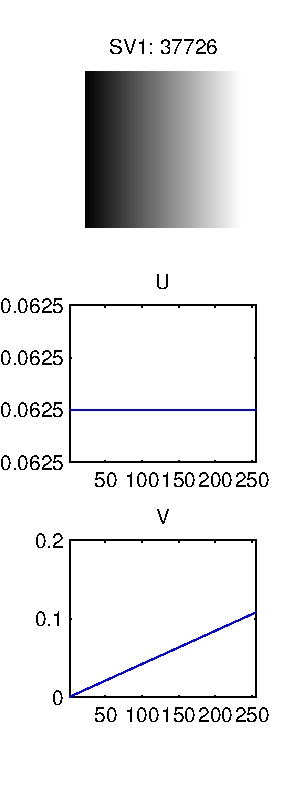
\includegraphics[width=\textwidth]{graphics/singular_vectors_gradient.pdf}
                \caption{Gradient}
        \end{subfigure}
        ~~~
        \begin{subfigure}[b]{0.2\textwidth}
                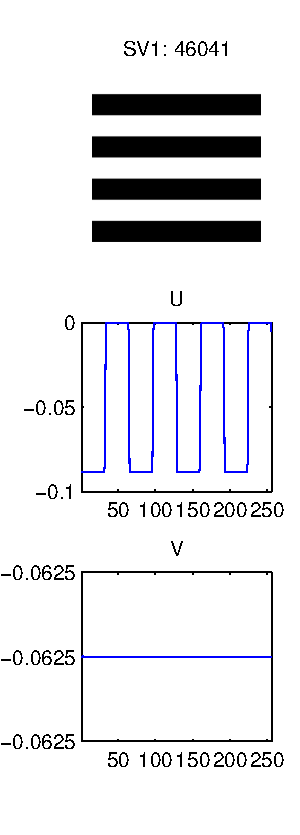
\includegraphics[width=\textwidth]{graphics/singular_vectors_horizontal.pdf}
                \caption{Vertical}
        \end{subfigure}
        ~~~
        \begin{subfigure}[b]{0.19\textwidth}
        		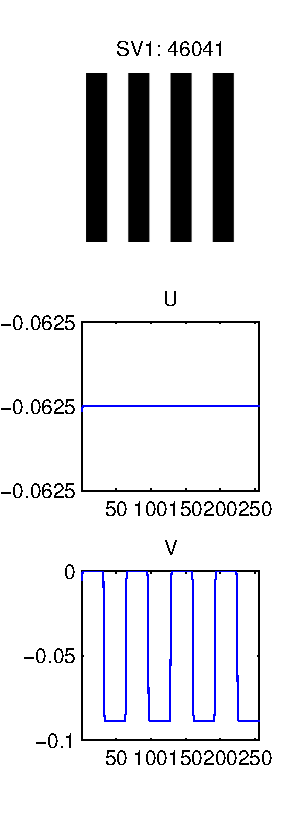
\includegraphics[width=\textwidth]{graphics/singular_vectors_vertical.pdf}
        		\caption{Horizontal}
        \end{subfigure}
        \caption{1st singular value composite image (top), left singular vector (mid), and right singular vector (bottom) }
        \label{fig:rank1_vectors}
\end{figure}

Figure \ref{fig:rank1_vectors} shows the first composite image that results from the multiplication of the first singular value by the first singular vectors. Since these images are rank 1, all other singular values are $0$ and are not shown. Variation of color in the horizontal direction is caused solely by singular vectors from V and variation in the vertical direction is caused by singular vectors from U. For low-rank matrices, the use of singular vectors as descriptors would preform well and would provide additional information above singular values (orientation of color change). However, similar to the problems summarized in Figure \ref{fig:rand_symmetry}, off-axis color change leads to much different results.

\begin{figure}[H]
        \centering
        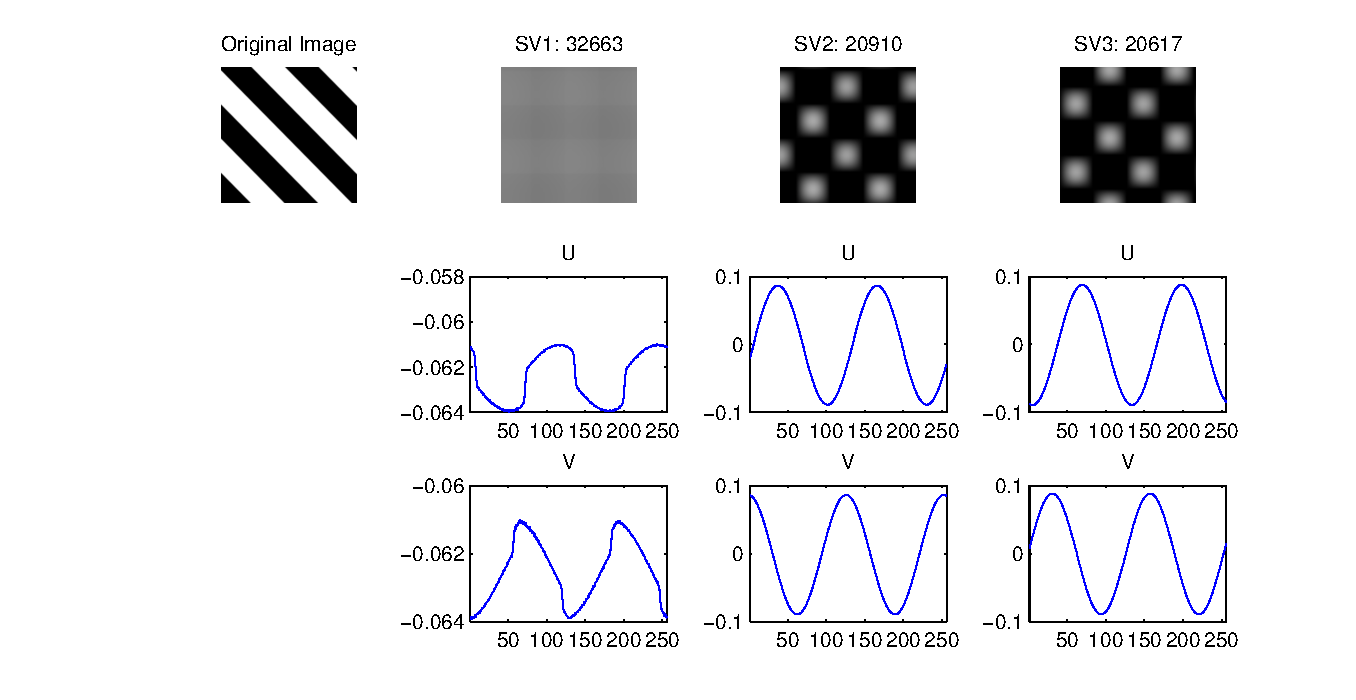
\includegraphics[width=\textwidth]{graphics/singular_vectors_diagonal.pdf}
        \caption{singular value composite image (top), left singular vector (mid), and right singular vector (bottom)}
        \label{fig:diagonal_vectors}
\end{figure}

Figure \ref{fig:diagonal_vectors} shows an example of worst case off-axis color change. Since color change does not align with either axis, the matrix is full rank and the decomposition requires all singular values. This case shows why a direct use of singular vectors to compare images (or singular values) is difficult. Although this image is arguable similar to the horizontal and vertical line images in Figure \ref{fig:rank1_vectors}, it has a much different decomposition.

\begin{figure}[H]
        \centering
        \begin{subfigure}[b]{0.48\textwidth}
                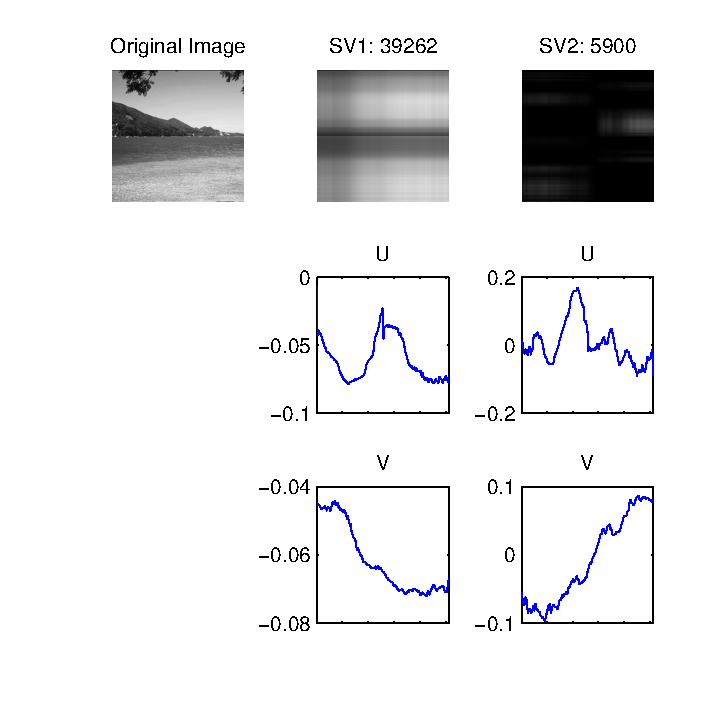
\includegraphics[width=\textwidth]{graphics/singular_vectors_coast.pdf}
                \caption{Coast}
        \end{subfigure}
        \begin{subfigure}[b]{0.48\textwidth}
                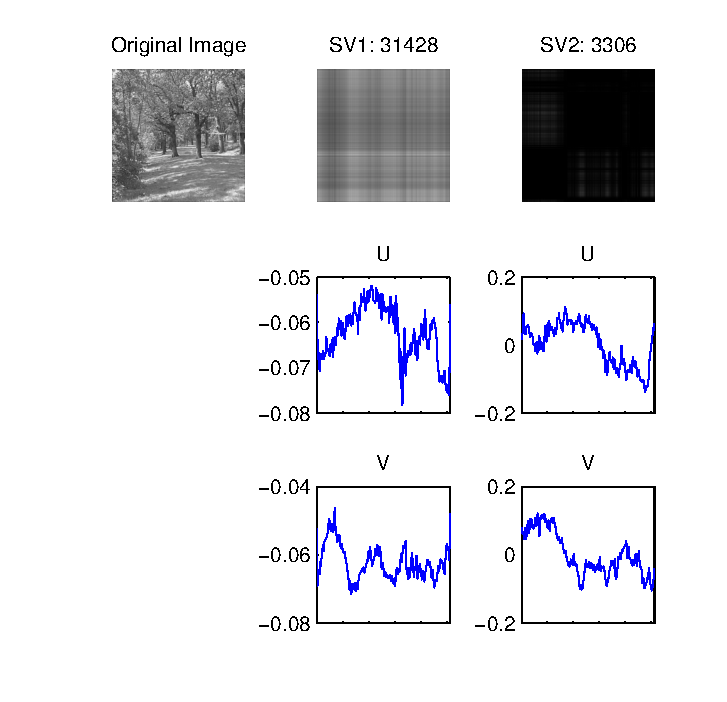
\includegraphics[width=\textwidth]{graphics/singular_vectors_forest.pdf}
                \caption{Forest}
        \end{subfigure}
        \caption{A comparison between top singular vectors and values of natural images}
        \label{fig:natural_vectors}
\end{figure}

Figure \ref{fig:natural_vectors} shows the top contributing singular vectors for a pair of natural images. The benefit of using singular vectors over singular values is again made clear here. Although the distribution of singular values is rather close between the two images (Figure \ref{fig:singular_values_natural}), the singular vectors capture an image's local variation as noise in their contribution. The coast has smooth transitions of color while the forest has sharp and frequent differences. This property gives an overall estimation of the complexity of structure in the image.

\subsection{A meaningful descriptor}

The distribution of singular values has been shown to provide a rough estimation of the amount of symmetry and repeated structure in an image, while doing little to capture more complex local structures. Singular vectors improve upon this to capture local variation as noise in the values of the vectors that contribute the most to an image's reconstruction. Both singular values and singular vectors are skewed by the fact that the decomposition depends heavily on image structure being aligned to the row bases or column bases.

To account for the effects of axis alignment, we simply take an image and rotate it by $45^\circ$ and $-45^\circ$ and concatenate descriptors for both the rotated and non-rotated images. The motivation for this construction being that if there is structure aligned along a line in the image (axis or off-axis), then a $45^\circ$ rotation will bring that closer to (or further from) an axis. Images with no linear structure should see little change from rotation.

To capture local noise in singular vectors we decide to take the FFT of the singular vectors rather than use them directly. This will capture the high frequency components of a noisy vector (such as the forest in \ref{fig:natural_vectors}) as well as the low frequency changes of a coastline or street.

\chapter{Analysis}
\label{chap:analysis}
[Steve] I suppose that here we should give a brief summary of k-means clustering and multidimensional scaling, and then show the results of the descriptor (with and without windowing) and an analysis of that? I was planning to investigate the properties of SVD and show some basic performance results in the SVD section....but that presents the problem that I evaluate my results with k-means and k-means won't be introduced yet..

E: I think we can introduce K-means, embedding, search by query, and any other similar things we used to test descriptors with in the Methods section, all under one section, say testing framework?


\chapter{Suggestions for Further Work}
%\subsection{Your Subsection title here}
%\subsubsection{Your subsubsection title here}
%\paragraph{Your paragraph title here}
Just some quick ideas - our exploration assumed that each property is indepenend which is obviously not true, and it would be interesting to look at similarities/ collerations between SVD and FT. 
Our exploration was purely based on properties of algorithms and visual exploration using MDS and k-nearest neighbour searches. Our performance for retrival is not really measured other that providing visual examples - some improvements on this front would be nice.
Images are extremly high dimensional space, and our analysis might not be entirely revealing - using some machine learning techniques (vide Zeyu and Shuran ) could help us to learn some more about mentioned dimensionality independence etc.
This project have not really focused on the color investigation very deeply where we have settled on euclidean distance between the RGB values. investigation of the non-linear distance metrics in HSV and Lab spaces might yield better results.

\begin{thebibliography}{6}

\bibitem{google_blog}
  Johanna Wright,
  \emph{Search by Text, Voice, or Image}.
  Inside Search: Official Google Search Blog,
  2011.
  
\bibitem{gist_descriptor}
  Aude Oliva, Antonio Torralba,
  \emph{	Modeling the Shape of the Scene: a Holistic Representation of the Spatial Envelope}.
  International Journal of Computer Vision, 
  Vol. 42(3): 145-175, 
  2001.

\bibitem{using_svd}
  Ientilucci, Emmett J,
  \emph{Using the singular value decomposition}. 
  Chester F. Carlson Center for Imaging Science,
  Rochester Institute of Technology,
  2003.

\bibitem{svd_image_coding}
  Andrews, Harry C. and Patterson, C., III,
  \emph{ Singular Value Decomposition (SVD) Image Coding}.
  IEEE Transactions on Communications,
  Vol. 24(4): 425-432,
  1976.

\bibitem{svd_image_retrieval}
  Jie-xian Zeng; Dong-ge Bi; Xiang Fu,
  \emph{A Matching Method Based on SVD for Image Retrieval}.
  Measuring Technology and Mechatronics Automation, 2009. ICMTMA '09. International Conference on, 
  Vol. 1: 396-398, 
  11-12 April 2009
  
\bibitem{color_model_ref}
  Agoston, Max K.
  \emph{Computer Graphics and Geometric Modelling: Mathematics}.
  Springer; 2005 edition,
  ISBN:1852338172
  
\bibitem{HSV_non_uniform}
    D. Androutsos and K. N. Plataniotis and A. N. Venetsanopoulos,
    \emph{A novel vector-based approach to color image retrieval using a vector angular-based distance measure},
    Computer Vision and Image Understanding,
    Vol. 75 : 46-58,
    1999
\bibitem{GaussQunatization}    
	Sangoh Jeong, Chee Sun Won, Robert M. Gray
	\emph{Image retrieval using color histograms generated by Gauss mixture vector quantization},
	Computer Vision and Image Understanding 
	Vol 94: 44-66,
	2004

\end{thebibliography}

\end{document}

